%!TEX TS-program = xelatex
%!TEX encoding = UTF-8 Unicode


\documentclass[11pt,twocolumn]{article}
\usepackage{geometry}
\usepackage{indentfirst}
\usepackage{authblk}
\usepackage{url}
\usepackage{graphicx}
\usepackage{subfigure}
\usepackage{amsmath}
\usepackage{listings}
\usepackage{color}
\usepackage{pgfplots}

 
\definecolor{codegreen}{rgb}{0,0.6,0}
\definecolor{codegray}{rgb}{0.5,0.5,0.5}
\definecolor{codepurple}{rgb}{0.58,0,0.82}
\definecolor{backcolour}{rgb}{0.95,0.95,0.92}
 
\lstdefinestyle{mystyle}{
    backgroundcolor=\color{backcolour},   
    commentstyle=\color{codegreen},
    keywordstyle=\color{magenta},
    numberstyle=\tiny\color{codegray},
    stringstyle=\color{codepurple},
    basicstyle=\footnotesize,
    breakatwhitespace=false,         
    breaklines=true,                 
    captionpos=b,                    
    keepspaces=true,                 
    numbers=none,                    
    numbersep=5pt,                  
    showspaces=false,                
    showstringspaces=false,
    showtabs=false,                  
    tabsize=2
}
 
\lstset{style=mystyle}
%\DeclareGraphicsExtensions{.pdf,.png,.jpg}

\geometry{letterpaper}


\usepackage{fontspec,xltxtra,xunicode}
\defaultfontfeatures{Mapping=tex-text}
\setromanfont{SimSun} %设置中文字体

\XeTeXlinebreaklocale “zh”
\XeTeXlinebreakskip = 0pt plus 1pt minus 0.1pt %文章内中文自动换行


\newfontfamily{\H}{SimHei}
\newfontfamily{\E}{Arial}  %设定新的字体快捷命令
\title{\H 基于CUDA的稀疏矩阵-向量乘法的实现}

\author{计算机学院\\吴振伟 (14060050)}
%\affil{计算机学院学员五队}
\date{}
%\date{\E\today}


\begin{document}
\maketitle

\renewcommand\abstractname{摘 要}
\begin{abstract}
稀疏矩阵-向量乘法(SpMV)是科学计算领域的一个基础问题。
因此,高效实现SpVM,对于提升科学计算问题求解性能至关重要。以GPU作为协处理单元提升计算机系统
并行数据处理能力的技术,今年来收到广泛关注。

本文对使用GPU加速SpVM求解的技术进行了系统学习和总结,并分别基于CPU和GPU对COO、CSR、ELL三种格式的计算性能进行了对别分析实验,得出ELL格式更适用于GPU计算的初步结论。\\
\end{abstract}

\noindent{\bf 关键词:} SpMV, GPU, CUDA

\section{引言}
众多科学计算问题,如线性方程组求解、偏微分方程求解等,均以稀疏矩阵-向量乘法(SpMV)为基础。高效实现SpMV,长期以来备受关注。

受限于工艺水平、材料物理特性、功耗等因素,单处理机性能提升达到极限。Intel, AMD等主流处理器厂商,均采用多核并行处理的技术,来提高处理器的整体运算性能。相应的,通过并行数据处理对大规模科学运算问题的优化,成为主流技术。

近年来,以通用图形处理单元(GPGPU)作为协处理部件,协同中央处理器(CPU)加速计算机系统对计算密集型程序的执行速度,引起了人们的广泛关注。
在市场需求的驱使下,传统的可编程图形处理单元(GPU)逐步发展成为具有强大运算能力和高度并行性的处理单元。GPGPU是指对图形处理器强大的并行处理能力和可编程流水线加以利用,协助中央处理器对非图形数据进行处理,即利用GPU对非图形相关的通用计算任务进行加速。

与CPU有所不同,GPU所采用的设计专门面向于具有高度并行性的数据密集型运算。GPU支持的硬件线程数,要远远大于多核CPU支持的硬件线程数。同一段程序在多组数据上并行执行,大大降低了运算过程的控制复杂性,并能够通过数据运算来隐藏访存延迟。这使得在GPU设计中,更多的硬件资源被专用于进行数据处理,而非用于数据缓存和程序流控制;使得GPU拥有相比CPU更加大的浮点运算能力和更高的存储器带宽。

NVIDIA公司于2007年提出了统一计算架构(Compute Unified Device Architecture, CUDA)~\cite{Nickolls:2008:SPP:1365490.1365500},该架构提供了一个清晰的GPU编程模型。
开发者可以基于CUDA,更加高效、充分地利用GPU的运算能力,对通用计算任务进行加速~\cite{Applications}。

本文接下来将分别对GPU和CUDA的架构进行简要介绍;
并对基于CUDA编程模型,实现稀疏矩阵-向量乘法的流程进行介绍。

\renewcommand{\figurename}{图}
\section{GPU硬件逻辑结构}
常见的多核心CPU的核数从几个到几十个不等,所支持的并发硬件线程数,在几个到几百个这样一个数量级。而常见的GPU器件,核心数达到几千个,并发硬件线程数远远超过CPU。GPU采用了一些特殊的设计和技术,来调度和管理如此大规模的并发线程。为了加深对GPU硬件结构的认识,这里不失一般性,以Nvidia公司开发的Fermi GPU微体系结构,如图~\ref{fig:fermi} ,对GPU的硬件逻辑结构进行简要的介绍~\cite{Fermi}。
\begin{figure}
  \centering
    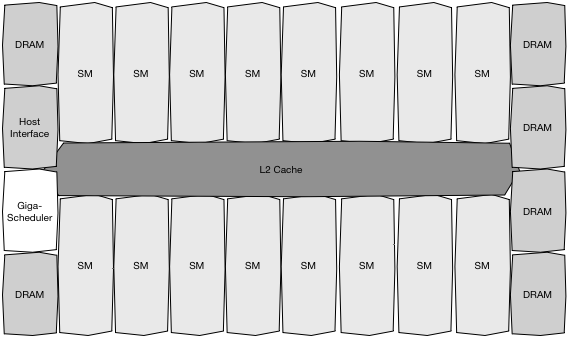
\includegraphics[scale=0.36]{images/hw-layout.png}
  \caption{Fermi微体系结构示意图}
  \label{fig:fermi}
\end{figure}

\begin{figure}
  \centering
    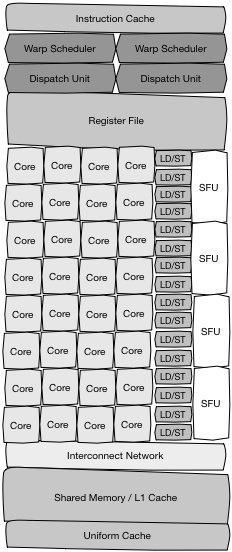
\includegraphics[scale=0.36]{images/sm-layout.png}
  \caption{多线程流处理器结构示意}
  \label{fig:sm-layout}
\end{figure}
GPU构建在一个多线程流式多核处理器(Streaming Multi-processors, SM)阵列之上。如图~\ref{fig:sm-layout}所示,每个SM又由32个处理器核心组成,即最大可以支持32个线程同时运行。在运行时,由GigaSchedular模块负责对任务进行粗粒度的调度——面向SM进行线程调度;SM中的WrapSchedular则负责更细粒度的调度——面向SM中的处理器核心进行线程调度。在下一小节中,本文将结合CUDA编程模型,分别对这两个粗粒度、和细粒度的调度过程,进行更加具体的描述。
%They guide the programmer to partition the problem into coarse sub-problems that can be solved independently in parallel by blocks of threads, and each sub-problem into finer pieces that can be solved cooperatively in parallel by all threads within the block.

\section{CUDA编程模型}
CUDA将线程抽象分组抽象为3个级别:由32个thread组成一个wrap;若干个wrap组成一个block;若干个block进而组成一个grid.

CUDA采用这样一种多层级、嵌套式的方式组织线程,获得了一种对软件开发过程透明的可扩展性。GPU以block为单位,对线程进行粗粒度调度:任意一个block可以被调度到任意一个可用的GPU内部的SM上运行。在SM内部,WrapSchedular又针对被调度的block中的若干个wrap,进行细粒度的调度。
在软件开发过程,编程人员通过上述线程组织结构对计算任务拆分进行描述。
这样一来,在CUDA框架下编写的程序,可以动态适应拥有任意处理器核心数的GPU。

GPU内部的SM,被设计成为SIMT(Single Instruction Multi-Thread)结构。在SIMT结构下,处理器以wrap为最小单位对线程进行调度和管理。当一个wrap被调度时,它所包含的32个thread从同一条指令开始执行;而每个thread拥有其独立的程序计数器和寄存器,所以同一个wrap中的多个thread可以自由进行分支跳转,相互独立地运行。在无跳转发生时,同一wrap中的所有thread共享执行路径;在有跳转发生时,处理器先后串行执行处于不同执行路径上的thread,直至所有分支路径最后又收敛到同一执行路径。忽略SIMT的这些处理细节,是可以保证程序的正确性的。而基于SIMT结构的这些特点,在编写thread代码时,有意识地规避掉执行路径出现分歧的情况,是提高程序性能的一个很好的切入点。
%Not all of the thousands or millions of threads actually run in parallel, but many do. Specifically, an NVIDIA GPU contains several largely independent processors called "Streaming Multiprocessors" (SMs), each SM hosts several "cores", and each "core" runs a thread.


\section{几种典型的稀疏矩阵存储格式}
针对稀疏矩阵中多数元素为0的这一特点,往往采用压缩存储的方式,实现更高效的存储。本节后续部分,将对几种常见的压缩方式如CSR、ELL等进行简要介绍\cite{Bell:SpMV:NVIDIA:2008}。
\subsection{几种典型的稀疏矩阵存储格式}
\subsubsection{DIA}
\begin{figure} 
  \centering 
  \subfigure{ 
    \label{fig:subfig:a} %% label for first subfigure 
    	$
		A = \begin{bmatrix}
				1 & 7 & 0 & 0         \\[0.3em]
				0 & 2 & 8 & 0         \\[0.3em]
				5 & 0 & 3 & 9         \\[0.3em]
				0 & 6 & 0 & 4
		\end{bmatrix}
		$
		}
  \hspace{3in} 
  \subfigure{ 
    \label{fig:subfig:b} %% label for second subfigure 
    	$
		data = \begin{bmatrix}
				* & 1 & 7         \\[0.3em]
				* & 2 & 8         \\[0.3em]
				5 & 3 & 9         \\[0.3em]
				6 & 4 & *
		\end{bmatrix}
		$
		$
		offsets = \begin{bmatrix}
				-2 & 0 & 1
		\end{bmatrix}
		$
    } 
  \caption{对角矩阵A的DIA表示} 
  \label{fig:DIA} %% label for entire figure 
\end{figure}

针对对角矩阵、分块对角矩阵等非零元素主要集中在主对角线附近区域的稀疏矩阵,
可以使用DIA格式实现高效存储。
如图~\ref{fig:DIA}所示:

DIA格式由data和offsets两部分组成。data矩阵中的一列,对应矩阵A中的一条非全零对角线,向量offsets一次存放了相应列编号相对主对角列编号的偏移量。
由于超对角线和次对角线上的元素少于主对角线元素,data矩阵中的相应列会出现空缺,应对的方案是分别在次对角线列和超对角线列的头部和尾部填充任意值。
这样一种处理方式,使得A中非零元的位置信息在data和offsets中得到充分描述——非零元在A矩阵中的行索引,等于其在data矩阵中的行索引;非零元在A矩阵的列索引,等于其行索引加上相应的偏移量。其总体效果是,实现了对数据的高效存储。
\subsubsection{ELLPACK}
\begin{figure} 
  \centering 
  \subfigure{ 
    \label{fig:subfig:a} %% label for first subfigure 
    	$
		A = \begin{bmatrix}
				1 & 7 & 0 & 0         \\[0.3em]
				0 & 2 & 8 & 0         \\[0.3em]
				5 & 0 & 3 & 9         \\[0.3em]
				0 & 6 & 0 & 4
		\end{bmatrix}
		$
		}
  \hspace{3in} 
  \subfigure{ 
    \label{fig:subfig:b} %% label for second subfigure 
    	$
		data = \begin{bmatrix}
				1 & 7 & *         \\[0.3em]
				2 & 8 & *         \\[0.3em]
				5 & 3 & 9         \\[0.3em]
				6 & 4 & *
		\end{bmatrix}
		$
		$
		indices = \begin{bmatrix}
				0 & 1 & * \\[0.3em]
				1 & 2 & * \\[0.3em]
				0 & 2 & 3 \\[0.3em]
				1 & 3 & * 
		\end{bmatrix}
		$
    } 
  \caption{对角矩阵A的ELL表示} 
  \label{fig:ELL} %% label for entire figure 
\end{figure}
ELLPACK(ELL)是一种更通用的存储方式,可应用于具有任何非零元分布形式的稀疏矩阵。如图~\ref{fig:ELL}所示:

ELL格式由data和indices两个矩阵组成。data矩阵中依次存放矩阵A中每一行的非零元,indices矩阵中依次存放相应的非零元在矩阵A中的列索引。
这种存储方式的空间开销,取决于矩阵A单行非零元个数的最大值。一个潜在的问题是,对于单行非零元最大值远远大于各行非零元平均值的矩阵,ELL存储方式将造成大量的空间浪费。
比如一个N节点星型网络的邻接矩阵,除中心点外,各个点的度为1,而中心点的度为N-1,这种情形就非常不适合使用ELL。


\subsubsection{COO}
\begin{figure} 
  \centering 
  \subfigure{ 
    \label{fig:subfig:a} %% label for first subfigure 
    	$
		A = \begin{bmatrix}
				1 & 7 & 0 & 0         \\[0.3em]
				0 & 2 & 8 & 0         \\[0.3em]
				5 & 0 & 3 & 9         \\[0.3em]
				0 & 6 & 0 & 4
		\end{bmatrix}
		$
		}
  \hspace{3in} 
  \subfigure{ 
    \label{fig:subfig:b} %% label for second subfigure 
    	$
		row = \begin{bmatrix}
				0 & 0 & 1 & 1 & 2 & 2 & 2 & 3 & 3 &
		\end{bmatrix}
		$
    }
  \subfigure{ 
    \label{fig:subfig:c} %% label for second subfigure 
    	$
		col = \begin{bmatrix}
				0 & 1 & 1 & 2 & 0 & 2 & 3 & 1 & 3 &
		\end{bmatrix}
		$
    }
  \subfigure{ 
    \label{fig:subfig:d} %% label for second subfigure 
    	$
		data = \begin{bmatrix}
				1 & 7 & 2 & 8 & 5 & 3 & 9 & 6 & 4 &
		\end{bmatrix}
		$
    } 
  \caption{对角矩阵A的COO表示} 
  \label{fig:COO} %% label for entire figure 
\end{figure}

Coordinate(COO)格式是一种非常简单、直观的稀疏矩阵存储格式。如图~\ref{fig:COO}所示:

由row、col、data三个向量,存放矩阵A中非零元的位置索引及其相应的值。

\subsubsection{CSR}
\begin{figure} 
  \centering 
  \subfigure{ 
    \label{fig:subfig:a} %% label for first subfigure 
    	$
		A = \begin{bmatrix}
				1 & 7 & 0 & 0         \\[0.3em]
				0 & 2 & 8 & 0         \\[0.3em]
				5 & 0 & 3 & 9         \\[0.3em]
				0 & 6 & 0 & 4
		\end{bmatrix}
		$
		}
  \hspace{3in} 
  \subfigure{ 
    \label{fig:subfig:b} %% label for second subfigure 
    	$
		ptr = \begin{bmatrix}
				0 & 2 & 4 & 7 & 9 &
		\end{bmatrix}
		$
    }
  \subfigure{ 
    \label{fig:subfig:c} %% label for second subfigure 
    	$
		indices = \begin{bmatrix}
				0 & 1 & 1 & 2 & 0 & 2 & 3 & 1 & 3 &
		\end{bmatrix}
		$
    }
  \subfigure{ 
    \label{fig:subfig:d} %% label for second subfigure 
    	$
		data = \begin{bmatrix}
				1 & 7 & 2 & 8 & 5 & 3 & 9 & 6 & 4 &
		\end{bmatrix}
		$
    } 
  \caption{对角矩阵A的CSR表示} 
  \label{fig:CSR} %% label for entire figure 
\end{figure}
与COO格式类似,Compressed sparse row(CSR)格式采用三个向量,显示地对非零元信息进行存储,如图~\ref{fig:CSR}。
区别在于对行索引的描述。对于一个行数为M的矩阵,CSR存放M+1个指针至向量ptr。前M个指针,分别记录每一行元素在indices和data向量中的起始偏移量;第M+1个指针存放的偏移量,等于第M行的偏移量与第M行非零元个数的和。

CSR存储方式在获得了一定的存储效率优化的同时,可以通过一个简单的减法运算(ptr[i+1]-ptr[i])来获得第i行非零元的总数,这一点带来了更多计算性能上的优化。
\section{基于CUDA实现SpMV}
基于CUDA编写的GPU并行程序,可以分为运行在CPU上的串行部分,和运行在GPU上的并行部分;以host代指CPU,以device代指GPU.运行在GPU上的线程,被称为kernel.将一个计算任务划分成若干个可以并行执行的子任务的过程,主要体现在对kernel的编写上。

图~\ref{fig:ell_kernel}展示了一个基于ELL格式的SpMV kernel的实现。其中,参数data和indices是两个一维数组的指针,分别指向ELL中的矩阵data和矩阵indices按照列优先次序组织成的一维数组。

kernel函数是对SIMT结构中,每个线程的行为描述。如图~\ref{fig:ell_kernel}中的kernel所示,在计算y=Ax时,每个线程计算y的一个分量,即计算矩阵A的某一行和向量x的内积。

由于矩阵data和矩阵indices按照列优先的方式组织为一维数组,同一个wrap内的多个线程对数组data和数组indices的访存地址是连续的。这一点有利于充分利用底层硬件的访存特性,实现联合访存,以提高访存效率。

\begin{figure} 
  \centering 
	\lstinputlisting[language=C++,basicstyle=\tiny]
	{example.c}
	\caption{SpMV ELL kernel} 
  	\label{fig:ell_kernel} %% label for entire figure 
\end{figure}

\section{实验验证}

\begin{figure} 
  	\centering 
	\subfigure[CPU]{ 
		\label{fig:result_CPU} %% label for first subfigure 
		\begin{tikzpicture}[scale=0.87,left]
		\begin{axis}[
			xticklabels={bcsstm12,bcsstk14,bcsstk25,af23560},xtick={1,...,5},
			%x tick label style={rotate=90,anchor=east},
			ylabel=Time(ms),
			enlargelimits=0.15,
			legend style={at={(0.5,-0.15)},anchor=north,legend columns=-1},
			%legend style={cells={anchor=north, fill}, nodes={inner sep=1,below=-1.1ex}},
			ybar,
			bar width=3pt,
		]

		%CPU time
		%COO 
		\addplot 
			coordinates {(1,4.16239977) (2,12.29318428) (3,48.62729645) (4,98.91919708)  };
		%CSR
		\addplot 
			coordinates {(1,2.59465599) (2,6.91289616) (3,27.00111961) (4,50.52972794) };
		%ELL
		\addplot 
			coordinates {(1,4.83225584) (2,12.91440010) (3,92.34770966) (4,83.81388855) };
		%\addplot[red,sharp plot,update limits=false] 
		%	coordinates {(1910,4.3e7) (1990,4.3e7)} ;
			%node[above] at (axis cs:1950,4.3e7) {Houses};
		\legend{COO,CSR,ELL}
		\end{axis}
		\end{tikzpicture}
	}
	\subfigure[GPU]{ 
		\label{fig:result_GPU} %% label for entire figure 
		\begin{tikzpicture}[scale=0.87,left]
		\begin{axis}[
			xticklabels={bcsstm12,bcsstk14,bcsstk25,af23560},xtick={1,...,5},
			%x tick label style={rotate=90,anchor=east},
			ylabel=Time(ms),
			enlargelimits=0.15,
			legend style={at={(0.5,-0.15)},anchor=north,legend columns=-1},
			%legend style={cells={anchor=north, fill}, nodes={inner sep=1,below=-1.1ex}},
			ybar,
			bar width=3pt,
		]
		\addplot 
			coordinates {(1,0.76815999) (2,0.56006402) (3,1.16822398) (4,1.97196805) };
		\addplot 	
			coordinates {(1,0.10508800) (2,0.21286400) (3,0.93919998) (4,2.23292804) };
		\addplot 	
			coordinates {(1,0.08476800) (2,0.15689600) (3,0.78688002) (4,0.46096000) };
		
		%\addplot[red,sharp plot,update limits=false] 
		%	coordinates {(1910,4.3e7) (1990,4.3e7)} ;
			%node[above] at (axis cs:1950,4.3e7) {Houses};
		\legend{COO,CSR,ELL}
		\end{axis}
		\end{tikzpicture}
	}
	\subfigure[Speed Up]{ 
		\label{fig:result_speedup} %% label for entire figure 
		\begin{tikzpicture}[scale=0.87,left]
		\begin{axis}[
			xticklabels={bcsstm12,bcsstk14,bcsstk25,af23560},xtick={1,...,5},
			%x tick label style={rotate=90,anchor=east},
			ylabel=Speed Up,
			enlargelimits=0.15,
			legend style={at={(0.5,-0.15)},anchor=north,legend columns=-1},
			%legend style={cells={anchor=north, fill}, nodes={inner sep=1,below=-1.1ex}},
			ybar,
			bar width=3pt,
		]
		\addplot 
			coordinates {(1,5.41866255) (2,21.94960594) (3,41.62497711) (4,50.16267776) };
		\addplot 
			coordinates {(1,24.69031525) (2,32.47564697) (3,28.74906349) (4,22.62935829) };
		
		\addplot 
			coordinates {(1,57.00566101) (2,82.31185150) (3,117.35932922) (4,181.82464600) };
	
		\legend{COO,CSR,ELL}
		\end{axis}
		\end{tikzpicture}
	} 
  	\caption{result} 
  	\label{fig:result} %% label for entire figure 
\end{figure}


这一部分对分别在CPU和NVIDIA GPU上基于COO、CSR、ELL这三种压缩格式实现SpMV的性能进行了对比分析实验。
实验矩阵测例来自Matrix Market~\cite{MatrixMarket},表~\ref{tab:tab_matrix}给出了这些矩阵测例的几个重要属性。
实验测试脚本见~\cite{wuzw}。实验基于2.3 GHz Intel Core i7 CPU和NVIDIA GeForce GT 650M 512 MB GPU, CUDA版本为V6.5.12.
实验过程中,仅针对计算过程对各测例进行时间测量~\cite{MetricsImplementation},未包括建立压缩格式的过程和CPU主存和GPU主存之间的数据拷贝过程。

图~\ref{fig:result_CPU}显示了分别基于COO、CSR、ELL三种存储格式,在CPU上实现SpMV的计算性能。
可以看出,CSR格式在CPU上相比其他两种格式,有较高的执行效率。
图~\ref{fig:result_GPU}则显示了三种格式在GPU上的性能表现。可以看出,在GPU上,ELL格式的性能表现更加突出。
基于上述实验结果计算得到的GPU相对CPU的加速比,在图~\ref{fig:result_speedup}中显示。

综上,可以得出一个初步的结论,CSR格式更适用于面向CPU的计算,而ELL格式则更适用于面向GPU计算。

\section{总结}
本学期,我选修了《高级计算机体系结构》这门课程,并在这门课上,第一次学习GPU体系结构。
出于对GPU加速的好奇,我选择了基于CUDA实验稀疏矩阵-向量乘法这样一个题目。
通过做这次课程报告,我对GPU的体系结构有了更加深入的认识。并掌握了基于CUDA面向GPU编程的基本技能。

当然,学无止境。基于CUDA实现GPU加速还远不止这么简单,还有很多更加深刻的内容值得去学习和探索,如更好的利用GPU存储层次结构
来对程序进行优化、通过改良kernel设计实现负载均衡等。

\section{致谢}
感谢成礼智教授的授课以及对科研经历的分享。他的敬业精神,为我树立了良好的榜样。

\renewcommand\refname{引用}
\bibliographystyle{ieeetr}
\bibliography{references}{}

\clearpage
\begin {table}[h]
\caption {实验矩阵属性~\cite{MatrixMarket}} \label{tab:tab_matrix} 

	\begin{tabular}{|p{2cm}|p{3cm}|p{2cm}|p{2cm}|p{2cm}|}
	\hline
	Matrix name              & size & nonzero & nonzero of longest row & nonzero of shortest row  \\
	\hline
	bcsstm12 & 1473 x 1473 & 19659 & 22 & 2   \\
	bcsstk14  & 1806 x 1806 & 63454 & 48 & 1    \\
	bcsstk25   & 15439 x 15439 & 252241 & 59 & 2  \\
	af23560    & 23560 x 23560 & 460598 & 21 & 9     \\
	\hline
	\end{tabular}
\end{table}

\end{document}